% !TeX spellcheck = en_US

\chapter{Introduction}
	
	problem: "things" get more complicated each day. additionally, these last years, repairing stuff has become nearly impossible.
	
	\begin{itemize}
		\itemsep0em
		\item mobile phones get less and less parts > even batteries are not replaceable anymore
		\item cars include expensive electronics in every single part
		\item solely from mechanical party consisting products are most likely made out of cheap irreplaceable plastic parts
	\end{itemize}
	
	solution:
	\begin{itemize}
		\itemsep0em
		\item find a professional (expensive)
		\item repair the thing yourself \begin{itemize}
			\itemsep0em
			\item with the help of the manufacture \begin{itemize}
				\item not really wanted > a repaired product last longer and shrinks profits from selling new product
				\item nowadays only for professional equipment (business laptops, ...)
					\begin{figure}[H]
						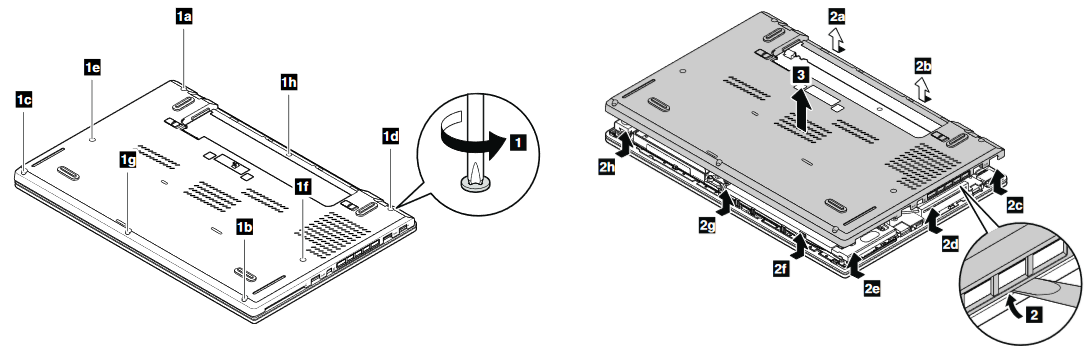
\includegraphics[width=\textwidth]{../images/common-manual.png}
						\centering
						\caption[adsf]{Typical step-by-step manual for business laptop hardware, taken from Hardware Maintainance Manual by Lenovo Thinkpad\footnotemark}
					\end{figure}
					\footnotetext{\url{https://download.lenovo.com/ibmdl/pub/pc/pccbbs/mobiles_pdf/t440s_hmm_en_sp40a25360_04.pdf}}
			\end{itemize}
			\item without the help of the manufacture \begin{itemize}
				\itemsep0em
				\item with technical skills > requirements increase drastically
				\item with no technical skills > manuals by other users (youtube videos, ...)
			\end{itemize}
		\end{itemize}
	\end{itemize}
	
	OUR solution:
	\begin{itemize}
		\itemsep0em
		\item \textbf{help user with repairing things by their own}
		\item new approach: use AR
		\item AR will come into the houses over the next years > device available
		\item AR devices are designed to show/add information to your environment and at the same time keep your hands free (alternation and interaction possible!) (not for tablets, ...) ...
	\end{itemize}
	
	
	section 2 will deal with the general product idea.
	
	section 3 takes a look at the specific problems that have to be faced because we use augmented reality
	
	section 4 checks possible business opportunities

